\chapter{Threads e Concorrenza}
Abbiamo già visto nell'introduzione una prima definizione di processo, l'entità attiva di un programma. Vediamo ora più nel dettaglio l'evoluzione di esso nel tempo.

\section{Thread}
Un thread è l'unità fondamentale della computazione, può essere generato da un processo aprendo la possibilità alla \textbf{parallelizzazione} della task.

\spacer
I thread appartenenti allo stesso processo condividono codice, dati e risorse (ad es. una modifica ad una variabile globale oppure l'apertura di un file sono visibili a tutti i thread)

Queste situazioni vanno però gestite correttamente, altrimenti si rischia di di avere conflitti nell'accesso alle risorse.

\begin{figure}[H]
    \centering
    \includegraphics[width=0.6\linewidth]{assets/multithread.jpg}
\end{figure}

\spacer

Il thread comprende:
\begin{sitemize}
    \item un identificatore di thread
    \item un contatore di programma
    \item un insieme di registri
    \item uno stack
\end{sitemize}

\begin{note}
    Il processo tradizionale, che viene eseguito su un singolo processo, si definisce "\textit{heavyweight process}", mentre i thread sono detti anche "processi leggeri".

    \spacer[4pt]

    Un thread può essere utilizzato dal browser per rappresentare una singola pagina web, per generare velocemente icone per una serie di immagini oppure possono essere usati da un webserver, un thread per ogni richiesta.
\end{note}

\subsection{Visualizzazione}

Per visualizzare lo stato di un processo in relazione al tempo useremo dei grafici con il tempo sull'asse x, e lo stato del processo sull'asse y.

\begin{figure}[H]
    \centering
    \begin{minipage}{0.45\textwidth}
        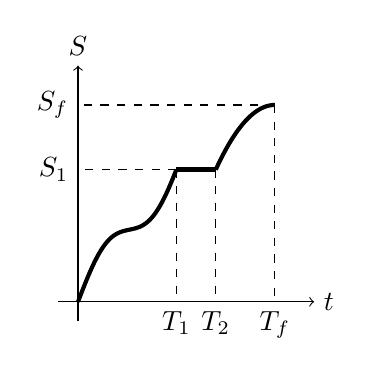
\begin{tikzpicture}[scale=2.5]
            % assi
            \draw[->] (-0.1,0) -- (1.2,0) node[right] {$t$};
            \draw[->] (0,-0.1) -- (0,1.2) node[above] {$S$};

            % funzioni
            \draw[domain=0:0.5,smooth,variable=\x, line width=1.5pt] plot ({\x},{1.4*\x+1/10*sin(deg(12*\x))});
            \draw[domain=0.5:0.7,smooth,variable=\x, line width=1.5pt] plot ({\x},{0.672});
            \draw[domain=0.7:1,smooth,variable=\x, line width=1.5pt] plot ({\x},{ -2.65 + 7.3*\x - 3.65*\x^2});

            % riferimenti
            \draw[dashed] (0.5,0.672) -- (0.5, 0)  node[below] {$T_1$};
            \draw[dashed] (0.7, 0.672) -- (0.7, 0) node[below] {$T_2$};
            \draw[dashed] (1, 1) -- (1, 0) node[below] {$T_f$};
            \draw[dashed] (0.5, 0.672) -- (0, 0.672) node[left] {$S_1$};
            \draw[dashed] (1, 1) -- (0, 1) node[left] {$S_f$};
        \end{tikzpicture}

        In questo caso particolare si può notare un periodo di tempo, da $T_1$ a $T_2$ dove il processo rimane nello stato $S_1$, questo indica che si trovava in un \textit{bottleneck}, ovvero il processo stava attendendo una qualche risorsa.
    \end{minipage}
    \hfill
    \begin{minipage}{0.45\textwidth}
        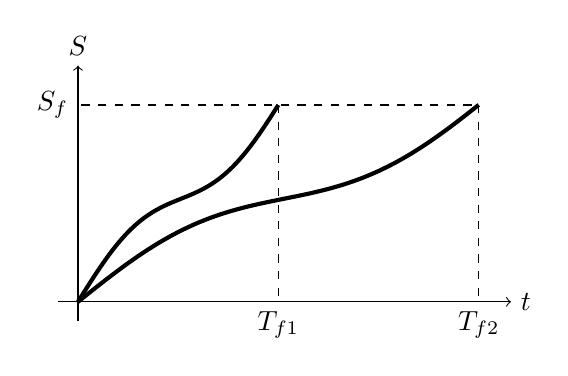
\begin{tikzpicture}[scale=2.5]
            % assi
            \draw[->] (-0.1,0) -- (2.2,0) node[right] {$t$};
            \draw[->] (0,-0.1) -- (0,1.2) node[above] {$S$};

            % funzioni
            \draw[domain=0:1.018,smooth,variable=\x, line width=1.5pt] plot ({\x},{\x+1/10*sin(deg(6*\x))});
            \draw[domain=0:2.036,smooth,variable=\x, line width=1.5pt] plot ({\x},{0.5*\x+1/10*sin(deg(3*\x))});

            % riferimenti
            \draw[dashed] (1.018, 1) -- (1.018, 0) node[below] {$T_{f1}$};
            \draw[dashed] (2.036, 1) -- (2.036, 0) node[below] {$T_{f2}$};
            \draw[dashed] (2, 1) -- (0, 1) node[left] {$S_f$};
        \end{tikzpicture}

        In questo casolo stesso processo viene eseguito su due processori diversi, $T_{f1}$ è il processore più veloce, mentre $T_{f2}$ quello più lento.
    \end{minipage}
\end{figure}

\subsection{User e Kernel Threads}
Nei moderni sistemi operativi esistono threads al livello utente e altri al livello kernel.
Quando un thread a livello utente fa una chiamata a sistema è necessario trovare un thread a livello kernel che sia pronto ad accettarla, altrimenti si rischia di introdurre dei tempi di attesa.
Va quindi trovata una relazione tra le due tipologie di threads.

\subsubsection{One-to-One}
Mappa ogni thread a livello utente con un suo corrispettivo a livello kernel, questo assicura che ogni \textit{systemcall} venga gestita correttamente e rapidamente.
Tuttavia così facendo si creano molti thread che potrebbero portare ad una riduzione delle prestazioni.

\begin{figure}[H]
    \centering
    \includegraphics[width=0.35\linewidth]{assets/one-to-one.jpg}
\end{figure}

\subsubsection{Many-to-Many}
Questo modello mappa $n$ thread utente a $k$ thread kernel, dove $n << k$. Questo modello ha una migliore utilizzazione delle risorse, ma è di difficile realizzazione la funzione che associa thread utente a thread kernel.
Ad oggi nessun sistema operativo moderno lo utilizza, si preferisce usare il modello one-to-one.

\begin{figure}[H]
    \centering
    \includegraphics[width=0.35\linewidth]{assets/many-to-many.jpg}
\end{figure}

\subsection{Implementazioni}
\subsubsection{Linux}
Linux implementa la Process Control Block mediante una \textit{task struct}, la ready queue diventa quindi una lista concatenata di \textit{task struct}.

\spacer
Quando un processo crea uno o più figli può scegliere se continuare la sua esecuzione in parallelo con essi o se attendere la loro conclusione.

Inoltre può scegliere se eseguire lo stesso codice del genitore o un altro programma.

\spacer
In linux, come in molti altri Sistemi Operativi, tutti i processi sono figli di un processo iniziale, nel caso di linux è il processo con ProcessID = 1.

Un nuovo processo viene generato con la funzione texttt{fork()} che restituisce l'id del nuovo processo al parent e restituisce 0 al figlio, questo è importante perché permettere di distinguere se ci si trova nel parent o nel children.

Quando il genitore non attende l'esecuzione dei figli e termina prima di essi essi sono detti \textbf{orfani} e alla loro terminazione diventano degli \textbf{zombie}.

\subsubsection{iOS}
Nelle prime versioni era previsto un solo processo utente in esecuzione.

A partire da iOS 4 vengono permessi anche dei processi di background, a priorità inferiore rispetto a quello di foregorund che ha il controllo della GUI.

\subsubsection{Android}
Le applicazioni che vogliono continuare l'esecuzione in background devono utilizzare un servizio.

\spacer
Quando dei processi devono essere terminati la selezione avviene secondo l'ordine:

processi vuoti -> background (non evidente all'utente) -> di servizio (evidente all'utente) -> visibile (usati da un processo foregorund) -> foregorund.

\subsubsection{Chrome}
Google chrome usa un processo di gestione del browser, dell'interfaccia utente, dell'I/O, poi utilizza un processo renderer per ogni pagina di navigazione.

\section{Programmazione multicore}
L'utilizzo di più thread si adatta naturalmente ai sistemi multicore, ma non solo, essa può trovare delle applicazioni anche in sistemi con un solo processore.

\subsection{Concorrenza}
La Concorrenza è l'esecuzione di più attività contemporaneamente, questo può essere ottenuto con un sistema multicore, oppure tramite uno scheduling efficiente dei cicli di un singolo processore.

\spacer
La concorrenza permette, almeno dal punto di vista dell'utente, di eseguire più processi contemporaneamente anche se questo può non essere vero.

Questo si ottiene tramite una grande quantità di \textit{context switch} da parte della CPU, che dedica ad ogni task una quantità di tempo infinitesimale.

Risulta quindi particolarmente importante scegliere correttamente le task che possono essere eseguite contemporaneamente e come sincronizzare.

\begin{figure}[H]
    \centering
    \includegraphics[width=0.65\linewidth]{assets/concorrenza.jpg}
    \caption{Concorrenza su un singolo processore}
\end{figure}

\subsection{Parallelismo}
Il parallelismo invece è la semplice esecuzione due o più task contemporaneamente. I due thread non devono necessariamente lavorare alla risoluzione dello stesso problema.
\begin{figure}[H]
    \centering
    \includegraphics[width=0.45\linewidth]{assets/parallelismo.jpg}
    \caption{Parallelismo su due processori}
\end{figure}

\spacer
Il parallelismo può essere implementato in vari modi:
\begin{itemize}
    \item \textbf{Parallelismo dei dati:}

          La stessa operazione viene eseguita contemporaneamente su processori diversi su segmenti diversi dei dati. (es. per analizzare 10 ore di registrazione, divido in elementi da 1 ora ciascuno)

    \item \textbf{Parallelismo delle task:}

          Significa distribuire i threads tra più processori, ogni thread esegue un'operazione differente. I thread possono lavorare sugli stessi dati, ma non è necessario.
\end{itemize}

\begin{figure}[H]
    \centering
    \includegraphics[width=0.45\linewidth]{assets/data-task-parallelism.jpg}
\end{figure}

\section{Sistemi di Processi}
È spesso conveniente scomporre un processo in $n$ sottoprocessi dando vita ad un sistema di processi, questo può permetterci di parallelizzare le operazioni pur rispettando l'ordine di esecuzione.

\begin{note}
    Possiamo utilizzare un grafo per rappresentare le relazioni di precedenza tra i processi, i nodi del grafo sono i sottoprocessi e un arco rappresenta una relazione di precedenza.
\end{note}

\subsubsection*{Esempio 4.1.}
Vogliamo risolvere l'equazione $f = (a + b) \cdot (c + d) + e$, possiamo risolverlo:
\begin{figure}[H]
    \centering
    \begin{minipage}{0.45\textwidth}
        \centering
        \includegraphics[width=\linewidth]{assets/math-sequenziale.jpeg}
        \caption{In modo sequenziale}
    \end{minipage}
    \hfill
    \begin{minipage}{0.35\textwidth}
        \centering
        \includegraphics[width=\linewidth]{assets/math-parallelo.jpeg}
        \caption{In parallelo}
    \end{minipage}
\end{figure}

\subsubsection*{Esempio 4.2.}
Conoscendo i tempi di esecuzione di ogni singolo processo possiamo anche calcolare la quantità di tempo che viene risparmiata parallelizzando l'operazione.

\begin{figure}[H]
    \centering
    \begin{minipage}{0.45\textwidth}
        \centering
        \includegraphics[width=\linewidth]{assets/threads-sequenziale.jpeg}
    \end{minipage}
    \hfill
    \begin{minipage}{0.35\textwidth}
        \centering
        \includegraphics[width=\linewidth]{assets/threads-parallelo.jpeg}
    \end{minipage}
    \caption{Aumento di efficienza ottenuto parallelizzando il processo}
\end{figure}

\subsection{Sistemi Chiusi e Aperti}

Un sistema si definisce \textbf{chiuso} se esiste un singolo processo iniziale e un singolo processo finale.

Il sistema è \textbf{aperto} se non è chiuso.

\spacer

Due sistemi di processi possono essere combinati in \textbf{serie} o in \textbf{parallelo}.

\begin{figure}[H]
    \centering
    \begin{minipage}{0.45\textwidth}
        \centering
        \includegraphics[width=\linewidth]{assets/sistema-serie.jpg}
    \end{minipage}
    \hfill
    \begin{minipage}{0.45\textwidth}
        \centering
        \includegraphics[width=\linewidth]{assets/sistema-parallelo.jpg}
    \end{minipage}
\end{figure}

\begin{note}
    I grafi ci permettono di trovare anche il \textbf{massimo grado di parallelismo} che un sistema raggiunge, si può trovare osservando il numero di processi nella stessa colonna.

    Nel caso rappresentato qui sopra ci sono al massimo 3 processi ponendo i sistemi in serie e 5 processi ponendo i sistemi in parallelo.
\end{note}

\subsection{Determinatezza}

Un sistema si dice \textbf{determinato} se le diverse velocità dei processi e l'ordine di esecuzione dei processi non influenzano il risultato.
Altrimenti si dice che il sistema è \textbf{indeterminato}.

\subsection{Inferenza}
\begin{note}
    Possiamo associare ad ogni processo un \textbf{dominio} contenente i dati su cui esso lavora e un \textbf{codominio} che contiene i risultati del processo.

    La \textbf{funzione mappa} trasforma elementi del dominio in elementi del codominio.
\end{note}

Due processi si dicono \textbf{non inferenti} se almeno una delle due osservazioni è corretta:
\begin{sitemize}
    \item Uno è il successore all'altro
    \item Non si intersecano i condomini e neppure i domini con i condomini.
\end{sitemize}

\subsubsection*{Proprietà}
\begin{sitemize}
    \item Condizione necessaria e sufficiente affinché un sistema sia \textbf{determinato} è che sia composto da processi \textbf{non inferenti}.
    \item Due sistemi sono \textbf{equivalenti} se sono costituiti dallo \textit{stesso insieme di processi}, sono \textit{determinati} e partendo dallo \textit{stesso input} producono lo \textit{stesso output}.
\end{sitemize}

\section{Risorse}
Diciamo \textbf{Risorsa} un'entità astratta, necessaria ad un processo per svolgere il proprio lavoro. Quando la risorsa non è disponibile il processo dovrà attendere per utilizzarla.

\spacer
Alcune risorse che sono \textbf{condivisibili} e possono essere usate da più processi in parallelo. Mentre alcune risorse possono essere usate da un solo processo allo stesso tempo.

\spacer
Un'altra classificazione delle risorse separa quelle non consumabili (es. un core), mentre altre sono \textbf{consumabili} (es. un dispositivo a batteria).

\spacer
Utilizziamo il termine \textbf{preemption} per definire la rimozione forzata di una risorsa ad un processo.

\subsection{Grafico dei Processi}

\begin{figure}[H]
    \centering
    \begin{minipage}{0.45\textwidth}
        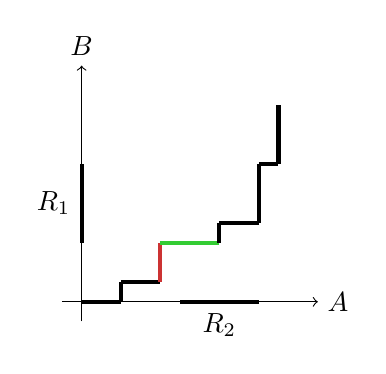
\begin{tikzpicture}[scale=2.5]
            % assi
            \draw[->] (-0.1,0) -- (1.2,0) node[right] {$A$};
            \draw[->] (0,-0.1) -- (0,1.2) node[above] {$B$};

            % grafico
            \draw[smooth, line width=1.5pt] (0, 0) -- (0.2, 0);
            \draw[smooth, line width=1.5pt] (0.2, 0) -- (0.2, 0.1);
            \draw[smooth, line width=1.5pt] (0.2, 0.1) -- (0.4, 0.1);
            \draw[smooth, line width=1.5pt, red!60!gray] (0.4, 0.1) -- (0.4, 0.3);
            \draw[smooth, line width=1.5pt, green!60!gray] (0.4, 0.3) -- (0.7, 0.3);
            \draw[smooth, line width=1.5pt] (0.7, 0.3) -- (0.7, 0.4);
            \draw[smooth, line width=1.5pt] (0.7, 0.4) -- (0.9, 0.4);
            \draw[smooth, line width=1.5pt] (0.9, 0.4) -- (0.9, 0.7);
            \draw[smooth, line width=1.5pt] (0.9, 0.7) -- (1, 0.7);
            \draw[smooth, line width=1.5pt] (1, 0.7) -- (1, 1);

            \draw[smooth, line width=1.5pt] (0, 0.3) -- (0, 0.5) node[left] {$R_1$};
            \draw[smooth, line width=1.5pt] (0, 0.5) -- (0, 0.7);
            \draw[smooth, line width=1.5pt] (0.5, 0) -- (0.7, 0) node[below] {$R_2$};
            \draw[smooth, line width=1.5pt] (0.7, 0) -- (0.9, 0);
        \end{tikzpicture}

        In questo caso i due processi A e B si alternano. Nel tratto rosso viene eseguito il processo B, mentre A è in attesa. Nel tratto verde accade l'opposto, il processo B che attende in favore di A.

        Le risorse $R_1$ e $R_2$ sono risorse non condivisibili, A usa $R_1$ e B $R_2$.

    \end{minipage}
    \hfill
    \begin{minipage}{0.45\textwidth}
        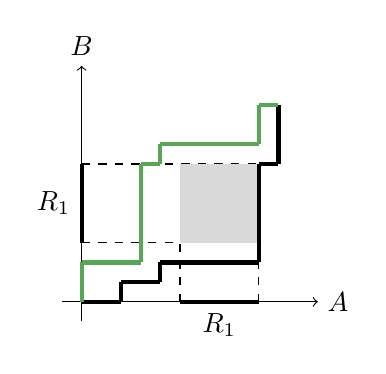
\begin{tikzpicture}[scale=2.5]
            % assi
            \draw[->] (-0.1,0) -- (1.2,0) node[right] {$A$};
            \draw[->] (0,-0.1) -- (0,1.2) node[above] {$B$};

            \draw[smooth, line width=1.5pt] (0, 0.3) -- (0, 0.5) node[left] {$R_1$};
            \draw[smooth, line width=1.5pt] (0, 0.5) -- (0, 0.7);
            \draw[smooth, line width=1.5pt] (0.5, 0) -- (0.7, 0) node[below] {$R_1$};
            \draw[smooth, line width=1.5pt] (0.7, 0) -- (0.9, 0);


            \draw[dashed] (0, 0.3) -- (0.5, 0.3);
            \draw[dashed] (0, 0.7) -- (0.9, 0.7);

            \draw[dashed] (0.5, 0) -- (0.5, 0.3);
            \draw[dashed] (0.9, 0) -- (0.9, 0.7);

            \draw[fill=gray!30, draw=none] (0.5,0.3) rectangle (0.9, 0.7);

            % grafico
            \draw[smooth, line width=1.5pt] (0, 0) -- (0.2, 0);
            \draw[smooth, line width=1.5pt] (0.2, 0) -- (0.2, 0.1);
            \draw[smooth, line width=1.5pt] (0.2, 0.1) -- (0.4, 0.1);
            \draw[smooth, line width=1.5pt] (0.4, 0.1) -- (0.4, 0.2);
            \draw[smooth, line width=1.5pt] (0.4, 0.2) -- (0.9, 0.2);
            \draw[smooth, line width=1.5pt] (0.9, 0.2) -- (0.9, 0.7);
            \draw[smooth, line width=1.5pt] (0.9, 0.7) -- (1, 0.7);
            \draw[smooth, line width=1.5pt] (1, 0.7) -- (1, 1);

            \draw[smooth, line width=1.5pt, green!30!gray] (0, 0) -- (0, 0.2);
            \draw[smooth, line width=1.5pt, green!30!gray] (0, 0.2) -- (0.3, 0.2);
            \draw[smooth, line width=1.5pt, green!30!gray] (0.3, 0.2) -- (0.3, 0.7);
            \draw[smooth, line width=1.5pt, green!30!gray] (0.3, 0.7) -- (0.4, 0.7);
            \draw[smooth, line width=1.5pt, green!30!gray] (0.4, 0.7) -- (0.4, 0.8);
            \draw[smooth, line width=1.5pt, green!30!gray] (0.4, 0.8) -- (0.9, 0.8);
            \draw[smooth, line width=1.5pt, green!30!gray] (0.9, 0.8) -- (0.9, 1);
            \draw[smooth, line width=1.5pt, green!30!gray] (0.9, 1) -- (1, 1);
        \end{tikzpicture}

        In questo caso invece i due processi devono condividere la stessa risorsa $R_1$, questo significa che il grafico non può mai entrare nell'area grigia.

        I due percorsi, nero e verde, sono entrambi validi per l'esecuzione dei due processi, entrambi passano al di fuori dell'area vietata.

    \end{minipage}
\end{figure}

\section{Deadlock}
Quando due processi richiedono la stessa risorsa non condivisibile, uno dei due attende l'altro.

\spacer
In alcuni casi però si può arrivare ad una situazione più complicata, ovvero quando due o più processi si attendono a vicenda, questo viene detto \textbf{deadlock} o \textbf{stallo}.

\spacer
Le condizioni necessarie (ma non sufficienti) per il verificarsi di un \textbf{deadlock}:
\begin{enumerate}
    \item Tutte le risorse devono essere non condivisibili.
    \item Il processo non ha un'unica operazione in cui richiede delle risorse.
    \item Al processo non può essere rimossa la risorsa, solo esso stesso può rilasciarla.
    \item L'attesa avviene in modo circolare, se ci sono $n$ processi, $P_1$ attende $P_2$, $\ldots$, $P_(n-1)$ attende $P_n$ e $P_n$ attende $P_1$.
\end{enumerate}

In questo caso ogni processo attende una risorsa che non verrà rilasciata, tutti attendono e nessuno può procedere.

\subsubsection*{Livelock}
Un sottoinsieme dei deadlock sono i livelock o stalli attivi, rappresenta una situazione dove i thread non sono effettivamente bloccati, ma effettivamente non progrediscono (es. due persone che si incontrano e si spostano ripetutamente da un lato all'altro del corridoio)

\subsection{Grafo delle Risorse}
Una visualizzazione utile per evidenziare possibili deadlock in fase di progettazione è il grafo delle risorse.

\spacer
I nodi del grafo rappresentano thread ($T_1, T_2, \ldots, T_n$) e risorse ($R_1, R_2, \ldots, R_n$), spesso vengono visualizzati in modo differente per distinguerli.

Diciamo \textit{arco di richiesta} $T_i -> R_j$ e un \textit{arco di assegnazione} $R_i -> T_j$

\spacer
A questo punto possiamo dire che se il grafo non contiene cicli chiusi allora non ci saranno deadlock. Quando invece il grafo contiene un ciclo e vi è una sola istanza per ogni risorsa allora ci sarà un deadlock, se almeno una risorsa ha più di un'istanza allora il deadlock è solamente possibile.

\begin{figure}[H]
    \centering
    \begin{minipage}{0.45\textwidth}
        \centering
        \includegraphics[width=0.65\linewidth]{assets/ciclo-deadlock.jpg}
        \caption{Situazione di deadlock}
    \end{minipage}
    \hfill
    \begin{minipage}{0.45\textwidth}
        \centering
        \includegraphics[width=0.9\linewidth]{assets/ciclo-no-deadlock.jpg}
        \caption{Situazione priva di deadlock}
    \end{minipage}
\end{figure}

\subsection{Prevenzione dei Deadlock}

\subsubsection{Allocazione globale}
Tutte le risorse richieste da un processo devono essere allocate prima che inizi l'esecuzione.

Questo garantisce l'assenza di deadlock, tuttavia è estremamente inefficiente reclamare tutte le risorse per tutto il periodo di esecuzione.

\subsubsection{Allocazione gerarchica}
Si assegna un ordine di importanza alle risorse, un processo può richiedere solo risorse più elevate di quelle che ha attualmente.
Se un processo necessita di una risorsa di priorità inferiore deve rilasciare quella attualmente in suo possesso per poi tornare a richiederla.

\begin{minipage}{0.45\textwidth}
    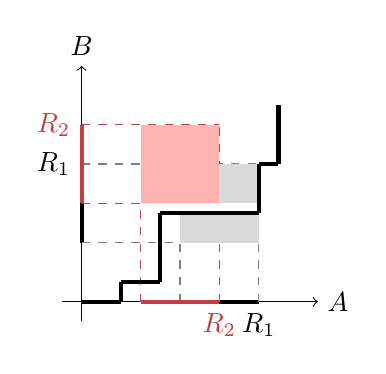
\begin{tikzpicture}[scale=2.5]
        % assi
        \draw[->] (-0.1,0) -- (1.2,0) node[right] {$A$};
        \draw[->] (0,-0.1) -- (0,1.2) node[above] {$B$};

        %R1
        \draw[smooth, line width=1.5pt] (0, 0.3) -- (0, 0.7) node[left] {$R_1$};
        \draw[smooth, line width=1.5pt] (0.5, 0) -- (0.9, 0) node[below] {$R_1$};


        \draw[dashed, gray] (0, 0.3) -- (0.5, 0.3);
        \draw[dashed, gray] (0, 0.7) -- (0.9, 0.7);

        \draw[dashed, gray] (0.5, 0) -- (0.5, 0.3);
        \draw[dashed, gray] (0.9, 0) -- (0.9, 0.7);

        %R2
        \draw[smooth, line width=1.5pt, red!50!gray] (0, 0.5) -- (0, 0.9) node[left] {$R_2$};
        \draw[smooth, line width=1.5pt, red!50!gray] (0.3, 0) -- (0.7, 0) node[below] {$R_2$};


        \draw[dashed, red!40!gray] (0, 0.5) -- (0.3, 0.5);
        \draw[dashed, red!40!gray] (0, 0.9) -- (0.7, 0.9);

        \draw[dashed, red!40!gray] (0.3, 0) -- (0.3, 0.5);
        \draw[dashed, red!40!gray] (0.7, 0) -- (0.7, 0.9);

        %squares
        \draw[fill=gray!30, draw=none] (0.5,0.3) rectangle (0.9, 0.7);
        \draw[fill=red!30, draw=none] (0.3,0.5) rectangle (0.7, 0.9);
        \draw[fill=white, draw=none] (0.3,0.45) rectangle (0.9, 0.5);

        % grafico
        \draw[smooth, line width=1.5pt] (0, 0) -- (0.2, 0);
        \draw[smooth, line width=1.5pt] (0.2, 0) -- (0.2, 0.1);
        \draw[smooth, line width=1.5pt] (0.2, 0.1) -- (0.4, 0.1);
        \draw[smooth, line width=1.5pt] (0.4, 0.1) -- (0.4, 0.45);
        \draw[smooth, line width=1.5pt] (0.4, 0.45) -- (0.9, 0.45);
        \draw[smooth, line width=1.5pt] (0.9, 0.45) -- (0.9, 0.7);
        \draw[smooth, line width=1.5pt] (0.9, 0.7) -- (1, 0.7);
        \draw[smooth, line width=1.5pt] (1, 0.7) -- (1, 1);
    \end{tikzpicture}
\end{minipage}

\subsubsection{Algoritmo del Banchiere}
Si impone che il thread $T_i$ inserisca nel grafo delle risorse tutti gli \textbf{archi di reclamo} a lui necessari prima di iniziare l'esecuzione.

Un arco di reclamo di un thread verso una risorsa indica al sistema che il thread utilizzerà in futuro quella risorsa. Un arco di reclamo diventa poi arco di richiesta in futuro.

\spacer
Definiamo \textbf{sequenza sicura} un ordinamento di n processi tali per lui le richieste di $P_i$ siano soddisfacibili dai processi $P_j$ con $j<i$

Uno \textbf{stato sicuro} è uno stato che contiene almeno una sequenza sicura.

\spacer
Per implementare l'algoritmo del banchiere vanno mantenute diverse strutture dati:
\begin{sitemize}
    \item Un \textbf{vettore $V$} che contiene il numero di istanze disponibili per ogni risorsa.
    \item Una \textbf{matrice $M$} che memorizza la massima quantità di istanze per ogni risorsa che viene usata dal thread.
    \item Una \textbf{matrice $R$} che memorizza le istanze per ogni risorsa attualmente allocate ad ogni thread.
    \item Una \textbf{matrice $N = M - R$}, che memorizza le risorse mancanti ad ogni thread.
\end{sitemize}

Tutte queste matrici devono essere aggiornate sia nei valori che nelle dimensioni.

\spacer
Per verificare che lo stato corrente sia sicuro deve essere possibile trovare almeno una sequenza di processi tale per cui sia possibile assegnare le risorse del vettore per completare ogni processo (le risorse necessarie al processo $i$ si trovano su $N[i]$)

\subsubsection{Algoritmo dello Struzzo}
L'algoritmo del banchiere deve essere eseguito frequentemente per poter rilevare i deadlock prima che si rivelino problematici, questo però richiede parecchie risorse del sistema.

\spacer
Per questo motivo molti sistemi \textit{consumer} \textbf{non} gestiscono i deadlock, essi avvengono in media una volta l'anno e in quel caso il sistema dovrà essere riavviato.

\subsection{Risoluzione di un Deadlock}
Una volta rilevato un deadlock per risolverlo ci sono due strategie spesso utilizzate.

\subsubsection{Terminazione dei Processi}
\begin{sitemize}
    \item Terminazione di tutti i processi che fanno parte del deadlock.

    Un sistema che risolve sicuramente il deadlock, ma viene anche ad un gran costo computazionale in quanto tutti i processi dovranno venir eseguiti da zero.

    \item Terminazione di un processo per volta finché il deadlock non viene rotto.
\end{sitemize}

\spacer
La scelta del processo da terminare è anch'essa gestita da un algoritmo che prende in considerare molti fattori, come la priorità del thread, il tempo di computazione trascorso, quantità di risorse che utilizza.


\subsubsection{Prelazione di Risorse}
Per risolvere il deadlock è anche possibile rimuovere risorse forzatamente ad uno o più processi.

Alcuni fattori da considerare quando si applica questa strategia sono:
\begin{sitemize}
    \item \textbf{Selezione della vittima}, è necessario scegliere un processo a cui rimuovere le risorse.
    \item \textbf{Rollback} dopo la rimozione della risorsa il thread non può continuare la sua esecuzione, è necessario tornare indietro a quando quella risorsa è stata acquisita.
    \item \textbf{Starvation} è importante non prelare le risorse sempre dallo stesso processo, altrimenti si potrebbe arrivare alla situazione in cui un processo non procede mai.
\end{sitemize}